\let\negmedspace\undefined
\let\negthickspace\undefined
\documentclass[journal,12pt,onecolumn]{IEEEtran}
\usepackage{cite}
\usepackage{amsmath,amssymb,amsfonts,amsthm}
\usepackage{algorithmic}
\usepackage{graphicx}
\usepackage{textcomp}
\usepackage{xcolor}
\usepackage{txfonts}
\usepackage{listings}
\usepackage{enumitem}
\usepackage{mathtools}
\usepackage{gensymb}
\usepackage{comment}
\usepackage[breaklinks=true]{hyperref}
\usepackage{tkz-euclide} 
\usepackage{gvv}                                        
%\def\inputGnumericTable{}                                 
\usepackage[latin1]{inputenc}     
\usepackage{xparse}
\usepackage{color}                                            
\usepackage{array}                                            
\usepackage{longtable}                                       
\usepackage{calc}                                             
\usepackage{multirow}
\usepackage{multicol}
\usepackage{hhline}                                           
\usepackage{ifthen}                                           
\usepackage{lscape}
\usepackage{tabularx}
\usepackage{array}
\usepackage{float}
\newtheorem{theorem}{Theorem}[section]
\newtheorem{problem}{Problem}
\newtheorem{proposition}{Proposition}[section]
\newtheorem{lemma}{Lemma}[section]
\newtheorem{corollary}[theorem]{Corollary}
\newtheorem{example}{Example}[section]
\newtheorem{definition}[problem]{Definition}
\newcommand{\BEQA}{\begin{eqnarray}}
\newcommand{\EEQA}{\end{eqnarray}}
\newcommand{\define}{\stackrel{\triangle}{=}}
\theoremstyle{remark}
\newtheorem{rem}{Remark}
% Marks the beginning of the document
\begin{document}
\title{gate}
\author{AI25btech11022 - Narshitha}
\maketitle
\renewcommand{\thefigure}{\theenumi}
\renewcommand{\thetable}{\theenumi}
\begin {center}
\large \textbf{2014}\\
\large \textbf{BT:Biotechnology}\\
\end{center}
\begin{enumerate}
    
    \item Choose the most appropriate word from the options given below to complete the following sentence.  

    A person suffering from Alzheimer's disease \_\_\_\_\_\_\_\_ short-term memory loss.  
\hfill \textbf{(GATE EE 2025)}
    \begin{enumerate} 
        \item experienced
        \item has experienced
        \item is experiencing
        \item experiences
    \end{enumerate}

    \item Choose the most appropriate word from the options given below to complete the following sentence.  

    \_\_\_\_\_\_\_\_ is the key to their happiness; they are satisfied with what they have.  \hfill \textbf{(GATE EE 2025)}

    \begin{enumerate} 
        \item Contentment
        \item Ambition
        \item Perseverance
        \item Hunger
    \end{enumerate}

    \item Which of the following options is the closest in meaning to the sentence below?  

   "As a woman, I have no country."
\hfill \textbf{(GATE EE 2025)}
    \begin{enumerate} 
        \item Women have no country.  
        \item Women are not citizens of any country.  
        \item Women's solidarity knows no national boundaries.  
        \item Women of all countries have equal legal rights.  
    \end{enumerate}

    \item In any given year, the probability of an earthquake greater than Magnitude 6 occurring in the Garhwal Himalayas is $0.04$. The average time between successive occurrences of such earthquakes is \_\_\_ years.  \hfill \textbf{(GATE EE 2025)}

    \begin{enumerate} 
        \item 3--4 years
        \item 4--5 years
        \item 5--6 years
        \item 6--7 years
    \end{enumerate}

    \item The population of a new city is $5$ million and is growing at 20\% annually. How many years would it take to double at this growth rate?  \hfill \textbf{(GATE EE 2025)}

    \begin{enumerate} 
        \item 3--4 years
        \item 4--5 years
        \item 5--6 years
        \item 6--7 years
    \end{enumerate}

    \item In a group of four children, Som is younger to Riaz. Shiv is elder to Ansu. Ansu is youngest in the group. Which of the following statements is/are required to find the eldest child in the group?  

    \textbf{Statements:}  \\
    1. Shiv is younger to Riaz.  \\
    2. Shiv is elder to Som.  \\ \hfill \textbf{(GATE EE 2025)}

    \begin{enumerate} 
        \item Statement 1 by itself determines the eldest child.  
        \item Statement 2 by itself determines the eldest child.  
        \item Statements 1 and 2 are both required to determine the eldest child.  
        \item Statements 1 and 2 are not sufficient to determine the eldest child.  
    \end{enumerate}

    \item Moving into a world of big data will require us to change our thinking about the merits of exactitude. To apply the conventional mindset of measurement to the digital, connected world of the twenty-first century is to miss a crucial point. As mentioned earlier, the obsession with exactness is an artefact of the information-deprived analog era. When data was sparse, every data point was critical, and this great care was taken to avoid letting any point bias the analysis.  

    From "BIG DATA" Viktor Mayer-Schonberger and Kenneth Cukier 

    The main point of the paragraph is:  
\hfill \textbf{(GATE EE 2025)}
    \begin{enumerate} 
        \item The twenty-first century is a digital world  
        \item Big data is obsessed with exactness  
        \item Exactitude is not critical in dealing with big data  
        \item Sparse data leads to a bias in the analysis  
    \end{enumerate}

    \item The total exports and revenues from the exports of a country are given in the two pie charts below.  
    (Pie charts show percentage distribution of quantity and revenue of exported items.)  

    The total quantity of exports of all the items is $5$ lakh tonnes and the total revenues are 250 crore rupees. What is the ratio of the revenue generated through export of Item 1 per kilogram to the revenue generated through export of Item 4 per kilogram?  
    \begin{figure}[H]
        \centering
        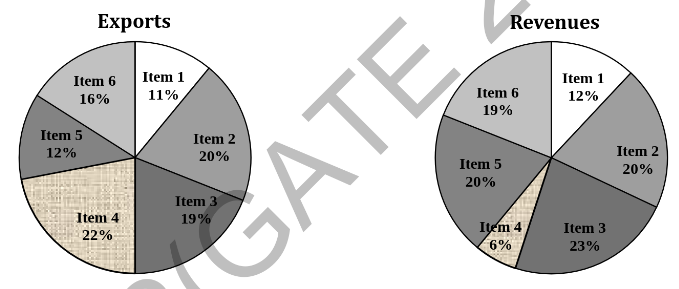
\includegraphics[width=0.5\linewidth]{figs/fig1.png}
        \caption{ }
        \label{fig1}
    \end{figure}
\hfill \textbf{(GATE EE 2025)}
    \begin{enumerate} 
        \item 1:2
        \item 2:1
        \item 1:4
        \item 4:1
    \end{enumerate}

    \item $X$ is 1 km northeast of $Y$. $Y$ is 1 km southeast of $Z$. $W$ is 1 km west of $Z$. $P$ is 1 km south of $Q$. $Q$ is 1 km east of $P$. What is the distance between $X$ and $Q$ in km?  \hfill \textbf{(GATE EE 2025)}

    \begin{enumerate} 
        \item 1
        \item $\sqrt{2}$
        \item $\sqrt{3}$
        \item 2
    \end{enumerate}

    \item 10\% of the population in a town is HIV$^+$. A new diagnostic kit for HIV detection is available; this kit correctly identifies HIV$^+$ individuals 95\% of the time, and HIV$^-$ individuals 95\% of the time. A particular patient is tested using this kit and is found to be positive. The probability that the individual actually is positive is \_\_\_.  \hfill \textbf{(GATE EE 2025)}
    \item The eigenvalues of 

A = $\myvec {1 & -4 \\ 2 & -3 }$

are \hfill \textbf{(GATE EE 2025)}
\begin{enumerate}
\item  $2 \pm i$
\item  $-1, -2$
\item  $-1 \pm 2i$
\item  non-existent
\end{enumerate}

\item If an unbiased coin is tossed 10 times, the probability that all outcomes are same will be $\_\_\_ \times 10^{-3}$
\hfill \textbf{(GATE EE 2025)}
\item The solution for the following set of equations is,
\[
\begin{aligned}
5x + 4y + 10z &= 13 \\
x + 3y + z &= 7 \\
4x - 2y + z &= 0
\end{aligned}
\] \hfill \textbf{(GATE EE 2025)}
\begin{enumerate}
\item  $x=2, y=1, z=1$
\item  $x=1, y=2, z=0$
\item  $x=1, y=0, z=2$
\item  $x=0, y=1, z=2$
\end{enumerate}

\item The limit of the function $e^{-2t}\sin(t)$ as $t \to \infty$, is \_\_\_
\hfill \textbf{(GATE EE 2025)}
\item  The solution to the following set of equations is,
\[
\begin{aligned}
2x + 3y &= 4 \\
4x + 6y &= 0
\end{aligned}
\] \hfill \textbf{(GATE EE 2025)}
\begin{enumerate}
\item  $x=0, y=0$
\item  $x=2, y=0$
\item  $2x = 4y = 6x$
\item  No solution
\end{enumerate}

\item The unit for specific substrate consumption rate in a growing culture is \hfill \textbf{(GATE EE 2025)}
\begin{enumerate}
\item  $\dfrac{g}{L \, h}$
\item  $\dfrac{g}{g \, h}$
\item  $\dfrac{g}{g \, h^2}$
\item  $\dfrac{gmoles}{L \, h}$
\end{enumerate}

\item If the dissociation constant for solute-adsorbent binding is $K_D$, the retention time of the solute in a chromatography column \hfill \textbf{(GATE EE 2025)}
\begin{enumerate}
\item  increases with increasing $K_D$
\item  decreases with increasing $K_D$
\item  passes through minimum with increasing $K_D$
\item  is independent of $K_D$
\end{enumerate}

\item In a batch culture of  Penicillium chrysogenum, the maximum penicillin synthesis occurs during the \hfill \textbf{(GATE EE 2025)}
\begin{enumerate}
\item  lag phase
\item  exponential phase
\item  stationary phase
\item  death phase
\end{enumerate}

\item The most plausible explanation for a sudden increase of the respiratory quotient (RQ) of a microbial culture is that \hfill \textbf{(GATE EE 2025)}
\begin{enumerate}
\item  cells are dying
\item  yield of biomass is increasing
\item  the fermentation rate is increasing relative to respiration rate
\item  the maintenance rate is decreasing
\end{enumerate}

\item  Which of the following is employed for the repeated use of enzymes in bioprocesses? \hfill \textbf{(GATE EE 2025)}
\begin{enumerate}
\item  polymerization
\item  immobilization
\item  ligation
\item  isomerization
\end{enumerate}

\item Since mammalian cells are sensitive to shear, scale-up of a mammalian cell process must consider, among other parameters, the following (given $N$ = rotations/time, $D$ = diameter of impeller) \hfill \textbf{(GATE EE 2025)}
\begin{enumerate}
\item  $\pi N D$
\item  $\pi N^2 D$
\item  $\pi N D^2$
\item  none of these
\end{enumerate}

\item  The degree of reduction of ethanol is \_\_\_\_ \hfill \textbf{(GATE EE 2025)}

\item  Gram-positive bacteria are generally resistant to complement-mediated lysis because \hfill \textbf{(GATE EE 2025)}
\begin{enumerate}
\item  thick peptidoglycan layer prevents insertion of membrane attack complex into the inner membrane
\item  Gram-positive bacteria import the membrane attack complex and inactivate it
\item  membrane attack complex is degraded by the proteases produced by the Gram-positive bacteria
\item  Gram-positive bacteria cannot activate the complement pathway
\end{enumerate}

\item A bacterium belonging to cocci group has a diameter of $2 \, \mu m$. The numerical value of the ratio of its surface area to volume (in $\mu m^{-1}$) is \_\_\_\_
\hfill \textbf{(GATE EE 2025)}

\item Which of the following essential element(s) is/are required as major supplement to enhance the bioremediation of oil spills by the resident bacteria? \hfill \textbf{(GATE EE 2025)} 
\begin{enumerate} 
\item Sulfur
\item Nitrogen and phosphorus
\item Iron
\item Carbon
\end{enumerate}

\item The 4-amino or 4-keto group of pyrimidine bases is located in the   \hfill \textbf{(GATE EE 2025)}
\begin{enumerate} 
\item major groove of the double stranded DNA
\item minor groove of the double stranded DNA
\item minor groove of the B form DNA but not the A form DNA
\item major groove of the B form DNA but not the A form DNA
\end{enumerate}

\item The product(s) resulting from the hydrolysis of maltose is/are   \hfill \textbf{(GATE EE 2025)}
\begin{enumerate} 
\item A mixture of $\alpha$-D-Glucose and $\beta$-D-Glucose
\item A mixture of D-Glucose and L-Glucose
\item $\alpha$-D-Glucose only
\item $\beta$-D-Glucose only
\end{enumerate}

\item Amino acid residue which is most likely to be found in the interior of water-soluble globular proteins is  \hfill \textbf{(GATE EE 2025)}
\begin{enumerate}
\item Threonine
\item Aspartic acid
\item Valine
\item Histidine
\end{enumerate}

\item The 5' ends of the mature forms of the prokaryotic mRNAs and tRNAs are \hfill \textbf{(GATE EE 2025)}  
\begin{enumerate} 
\item a triphosphate group in mRNAs and a monophosphate group in tRNAs
\item triphosphate groups in both mRNAs and tRNAs
\item monophosphate groups in both mRNAs and tRNAs
\item a monophosphate group in mRNAs and a triphosphate group in tRNAs
\end{enumerate}

\item Prior exposure of plants to pathogens is known to increase resistance to future pathogen attacks. This phenomenon is known as \hfill \textbf{(GATE EE 2025)} 
\begin{enumerate} 
\item systemic acquired resistance
\item hypersensitive response
\item innate immunity
\item antibody mediated response
\end{enumerate}

\item Reactions between antibodies and antigens that are detected by precipitate formation in an agar gel are referred as  \hfill \textbf{(GATE EE 2025)}
\begin{enumerate} 
\item immunoprecipitation assay
\item immunodiffusion assay
\item immunoaggregation assay
\item immunofixation assay
\end{enumerate}

\item The algorithm for BLAST is based on  \hfill \textbf{(GATE EE 2025)}
\begin{enumerate} 
\item Dynamic Programming
\item Hidden Markov Model
\item K-tuple analysis
\item Neural Network
\end{enumerate}

\item The statistical frequency of the occurrence of a particular restriction enzyme cleavage site that is 6 bases long can be estimated to be  \hfill \textbf{(GATE EE 2025)}
\begin{enumerate} 
\item once every 24 bases
\item once every 256 bases
\item once every 1024 bases
\item once every 4096 bases
\end{enumerate}

\item The reactions leading to the formation of amino acids from the TCA cycle intermediates are  \hfill \textbf{(GATE EE 2025)}
\begin{enumerate} 
\item carboxylation
\item isomerization
\item transamination
\item decarboxylation
\end{enumerate}

\item The growth medium for mammalian cells contains serum. One of the major functions of serum is to stimulate cell growth and attachment. However, it must be filter sterilized to  \hfill \textbf{(GATE EE 2025)}
\begin{enumerate} 
\item remove large proteins
\item remove collagen only
\item remove mycoplasma and microorganisms
\item remove foaming agents
\end{enumerate}
\item The concentration profile of a chemical at a location $x$ and time $t$, denoted by $c(x,t)$, changes as per the following equation,
\[
c(x,t) = \frac{c_0}{\sqrt{2 \pi D t}} \exp \left( - \frac{x^2}{2Dt} \right)
\]
where $D$ and $c_0$ are assumed to be constant. Which of the following is correct? \hfill \textbf{(GATE EE 2025)}
\begin{enumerate}
\item  $\dfrac{\partial c}{\partial t} = D \dfrac{\partial^2 c}{\partial x^2}$
\item  $\dfrac{\partial c}{\partial t} = 2D \dfrac{\partial^2 c}{\partial x^2}$
\item  $\dfrac{\partial^2 c}{\partial t^2} = D \dfrac{\partial^2 c}{\partial x^2}$
\item  $\dfrac{\partial c}{\partial t} = \dfrac{\partial^2 c}{\partial x^2}$
\end{enumerate}

\item If $y = x^x$, then $\dfrac{dy}{dx}$ is \hfill \textbf{(GATE EE 2025)}
\begin{enumerate}
\item  $x^x(x-1)$
\item  $x^{x-1}$
\item  $x^x (1 + \log x)$
\item  $e^x (1 + \log x)$
\end{enumerate}

\item  Which of the following statements is true for the series given below?
\[
s_n = 1 + \frac{1}{\sqrt{2}} + \frac{1}{\sqrt{3}} + \cdots + \frac{1}{\sqrt{n}}
\] \hfill \textbf{(GATE EE 2025)}
\begin{enumerate}
\item  $s_n$ converges to $\log (\sqrt{n})$
\item  $s_n$ converges to $\sqrt{n}$
\item  $s_n$ converges to $\exp (\sqrt{n})$
\item  $s_n$ diverges
\end{enumerate}

\item  The graph of the function $F(x)= \dfrac{1}{k_1x^{2}+k_2x +1}$ for $0<x<\infty$ is \hfill \textbf{(GATE EE 2025)}  
\begin{figure}[H]
    \centering
    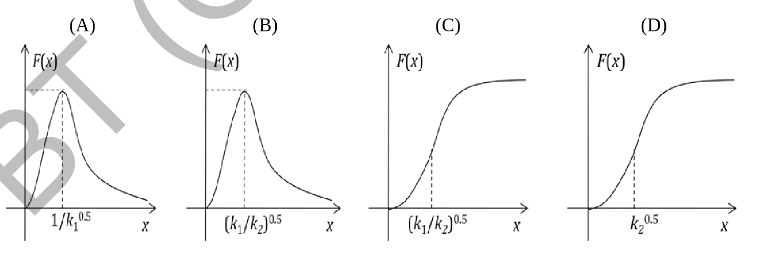
\includegraphics[width=0.6\linewidth]{figs/fig2.png}
    \caption{ }
    \label{fig2}
\end{figure}

\item  A T-flask is seeded with $10^5$ anchorage-dependent cells. The available area of the T-flask is 25 cm$^2$ and the volume of the medium is 25 ml. Assume that the cells are rectangles of size $5 \,\mu m \times 2 \,\mu m$. If the cells grow to monolayer confluence after 50 h, the growth rate in number of cells/(cm$^2\cdot$h) is \_\_\_ $\times 10^3$. \hfill \textbf{(GATE EE 2025)}
\item  Consider a continuous culture provided with a sterile feed containing 10 mM glucose. The steady state cell density and substrate concentration at three different dilution rates are given in the table below:

\[
\begin{array}{|c|c|c|}
\hline
\text{Dilution rate (h$^{-1}$)} & \text{Cell density (g/L)} & \text{Substrate conc. (mM)} \\
\hline
0.05 & 0.248 & 0.067 \\
0.5 & 0.208 & 1.667 \\
5 & 0.0 & 10.0 \\
\hline
\end{array}
\]

The maximum specific growth rate $\mu_m$ (in h$^{-1}$), will be \_\_\_.
\hfill \textbf{(GATE EE 2025)}
\item  Cholera toxin increases cAMP levels by
\begin{enumerate}
\item  modifying G protein
\item  modifying GTP
\item  binding to adenylate cyclase
\item  activating cAMP phosphodiesterase
\end{enumerate}

\item  Triose phosphate isomerase converts dihydroxy acetone phosphate (DHAP) to glyceraldehyde-3-phosphate (G-3-P) in a reversible reaction. At 298 K and pH 7.0, the equilibrium mixture contains 40 mM DHAP and 4 mM G-3-P. Assume that the reaction started with 44 mM DHAP and no G-3-P. The standard free-energy change in kJ/mol for the formation of G-3-P ($R=8.315$ J/mol·K) is \_\_. \hfill \textbf{(GATE EE 2025)}

\item  The plasmid DNA was subjected to restriction digestion using the enzyme  EcoRI and analysed on an agarose gel. Assuming digestion has worked (the enzyme was active), match the identity of DNA bands shown in the image in Group I with their identity in Group II.
\begin{figure}[H]
    \centering
    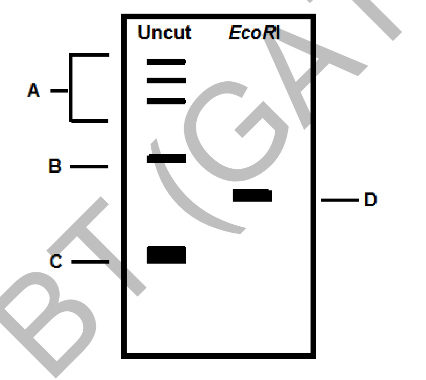
\includegraphics[width=0.4\linewidth]{figs/fig3.png}
    \caption{ }
    \label{fig3}
\end{figure}
\begin{tabular}{c c} 
      
\textbf{Group I} & \textbf{Group II}\\
P. Band labeled as A &   1. Nicked\\
Q. Band labeled as B &   2. Supercoiled\\
R. Band labeled as C &   3. Concatemers\\
S. Band labeled as D &  4. Linear\\
\end{tabular}

\hfill \textbf{(GATE EE 2025)}
\begin{enumerate}
\item  P-3, Q-1, R-2, S-4
\item  P-1, Q-4, R-3, S-2
\item  P-4, Q-3, R-2, S-1
\item  P-4, Q-1, R-3, S-2
\end{enumerate}

\item In a relatively large but finite and closed population of sexually reproducing diploid organisms, the frequency of homozygous genotype PP changes from 0.40 to 0.50 and that of Pp changes from 0.40 to 0.41 in a span of 10 generations. Which of the following is the most likely cause for the above change in frequency of the PP genotype? \hfill \textbf{(GATE EE 2025)}
\begin{enumerate} 
\item Non-random mating
\item Random genetic drift
\item Selection
\item Combination of non-random mating and random genetic drift
\end{enumerate}

\item Topological winding number of a 2.0 kb covalently closed circular DNA was found to be 191 with a writhing number of -4. Hence, its LINKING NUMBER and the NUMBER OF BASE PAIR PER TURN when the molecule is laid flat on the surface is \underline{\hspace{2cm}} and \underline{\hspace{2cm}}, respectively. \hfill \textbf{(GATE EE 2025)}
\begin{enumerate} 
\item 187, 10.69
\item 195, 10.25
\item 200, 10.00
\item 187, 10.50
\end{enumerate}

\item Consider a population of 10,000 individuals, of which 2500 are homozygotes (PP) and 3000 are heterozygotes (Pp) genotype. The frequency of allele p in the population is \underline{\hspace{2cm}}. \hfill \textbf{(GATE EE 2025)}

\item Match the following photoreceptors with their prosthetic groups and spectral specificity \\
\begin{tabular}{c c c}
    

\textbf{Photoreceptor} & \textbf{Moiety that absorbs light} & \textbf{Absorption (nm)}\\
P. Phototropin & 1.Chromobilin & a. 400--500 \\
Q. Cryptochrome & 2. FAD & b. 600--800 \\
R. Phytochrome & 3. FMN & c. 500--600 \\


\end{tabular} \hfill \textbf{(GATE EE 2025)}
\begin{enumerate} 
\item P-3, Q-2, R-1; a-b
\item P-1, Q-2, R-3; b-a-c
\item P-3, Q-2, R-1; c-a
\item P-2, Q-1, R-1; a-b
\end{enumerate}

\item Match the following plant sources with their secondary metabolites and medical uses \\
\begin{tabular}{c c c}

\textbf{Source plant} & \textbf{Secondary metabolites} & \textbf{Medical uses}\\
P. Belladonna &1. Menthol & a.Cancer treatment  \\
Q. Foxglove & 2. Atropine & b. Heart disease \\
R. Pacific & 3. Digitalin & c. Eye treatment \\
S. Eucalyptus & 4. Taxol & d.  Cough\\
\end{tabular} \hfill \textbf{(GATE EE 2025)}
\begin{enumerate} 
\item P-2-c, Q-3-b, R-4-c, S-5-d
\item P-1-b, Q-4-c, R-2-d, S-3-a
\item P-2-c, Q-4-b, R-1-a, S-3-d
\item P-1-b, Q-4-c, R-2-d, S-3-a
\end{enumerate}

\item The pungency of mustard seeds is primarily due to secondary metabolites such as isothiocyanate and nitrile. The pungency is usually felt only when the seeds are crushed. This is because of \hfill \textbf{(GATE EE 2025)}
\begin{enumerate} 
\item the coat of the intact seeds blocks the pungent volatiles from being released
\item the pungent chemicals are stored as inactive conjugates and compartmentalized from the enzymes that convert them into active chemicals
\item the pungent chemicals are formed only after the reaction with atmospheric oxygen
\item the pungent chemicals are formed only after the reaction with atmospheric carbondioxide
\end{enumerate}

\item In a mouse genome, the numbers of functional $V_\alpha$, $J_\alpha$, $V_\beta$, $D_\beta$, $J_\beta$ gene segments are 79, 38, 21, 2 and 11, respectively. The total number of possible combinations for $\alpha\beta$ T cell receptors are \underline{\hspace{2cm}} $\times 10^6$. \hfill \textbf{(GATE EE 2025)}



\item The percentage SIMILARITIES and IDENTITIES, respectively, between the two peptide sequences given below will be \underline{\hspace{1cm}} \% and \underline{\hspace{1cm}} \%.
\\
Peptide I : Ala-Ala-Arg-Arg-Gln-Trp-Leu-Thr-Phe-Thr-Lys-Ile-Met-Ser-Glu \\
Peptide II: Ala-Ala-Arg-Glu-Gln-Tyr-Ile-Ser-Phe-Thr-Lys-Ile-Met-Arg-Asp\\
\hfill \textbf{(GATE EE 2025)}
\begin{enumerate} 
\item  80, 80
\item  80, 60
\item  60, 60
\item  90, 60
\end{enumerate}

\item In an affine gap penalty model, if the gap opening penalty = 20, gap extension penalty = 4 and gap length is 8, the gap score is \underline{\hspace{2cm}}.
\hfill \textbf{(GATE EE 2025)}
\item For their efficient translation, eubacterial mRNAs possess a Shine-Dalgarno sequence for its recognition by an anti-Shine-Dalgarno sequence (ASD) in the ribosomes. The correct statement is \hfill \textbf{(GATE EE 2025)}
\begin{enumerate} 
\item ASD is present in 5S rRNA
\item ASD is present in 23S rRNA
\item ASD is present in 16S rRNA
\item ASD is formed by the interaction of the 16S rRNA with the 23S rRNA upon docking of the 50S subunit on the 30S subunit of the ribosomes
\end{enumerate}

\item Match the items in Group I with Group II\\
\begin{tabular}{c c}

\textbf{Group I} & \textbf{Group II} \\
P. Receptor tyrosine kinase & 1. Inactivation of G-proteins \\
Q. Cyclic GMP (cGMP) & 2. Reception of insulin signal \\
R. GTPase activating protein (GAP) & 3. Thyroid hormone \\
S. Nuclear receptor & 4. Receptor guanylyl cyclase \\
\end{tabular} \hfill \textbf{(GATE EE 2025)}
\begin{enumerate} 
\item P-1, Q-3, R-4, S-2
\item P-2, Q-4, R-3, S-1
\item P-3, Q-1, R-4, S-2
\item P-2, Q-4, R-1, S-3
\end{enumerate}

\item Match the immunoglobulin class in Group I with its properties in Group II\\
\begin{tabular}{c c}
\textbf{Group I} & \textbf{Group II} \\
P. IgG & 1. Major antibody in external secretions such as bronchial mucus \\
Q. IgA & 2. Protects against parasites \\
R. IgE & 3. Antibody that appears first in serum after exposure to an antigen \\
S. IgM & 4. Antibody present in highest concentration in serum \\

\end{tabular} \hfill \textbf{(GATE EE 2025)}
\begin{enumerate} 
\item P-4, Q-1, R-2, S-3
\item P-4, Q-3, R-1, S-2
\item P-3, Q-2, R-1, S-4
\item P-4, Q-1, R-3, S-2
\end{enumerate}



\item In a genetic cross between the genotypes WWXX and wwxx, the following phenotypic distributions were observed among the F$_2$ progeny: WX, 562; wx, 158; Wx, 38; and wX, 42. Likewise, a cross between XXYY and xxyy yielded the following results: XY, 675; xy, 175; Xy, 72; and xY, 78. Similarly, a cross between WWYY and wwyy yielded: WY, 292; wy, 88; Wy, 12; and wY, 8. In all the genotypes, capital letters denote the dominant allele. Assume that the F$_1$ progeny were self-fertilized in all three crosses. Also, double cross-over does not occur in this species. Which of the following is correct?  
\hfill \textbf{(GATE EE 2025)}
\begin{enumerate}
\item Relative position W-X-Y Distances: W-X = 5 map units, X-Y = 17 map units  
\item Relative position X-Y-W Distances: X-Y = 15 map units, Y-W = 11 map units  
\item Relative position Y-W-X Distances: Y-W = 5 map units, W-X = 11 map units  
\item Relative position X-W-Y Distances: X-W = 5 map units, W-Y = 10 map units  
\end{enumerate}


\item The length of the minimum unique stretch of DNA sequence that can be found only once in a 3 billion base pairs long genome is  
\hfill \textbf{(GATE EE 2025)}

\begin{enumerate}
\item 14  
\item 15  
\item 16  
\item 18  
\end{enumerate}


\item Lysine is being produced in a lab-scale reactor by a threonine auxotroph. After 2 weeks of operation it was observed that the concentration of lysine in the reactor was gradually decreasing. Microbiological assays of reactor samples showed absence of contamination and reactor condition showed no change in the operating conditions. The most probable reason for decrease in lysine concentration may be attributed to  
\hfill \textbf{(GATE EE 2025)}
 
\begin{enumerate} 
\item accumulation of ethanol  
\item growth of revertants  
\item production of citric acid  
\item utilization of lysine for cell growth  
\end{enumerate}
 

\item If a tumor is shifted to cold temperature, which of the following changes would take place in its membrane?  \hfill \textbf{(GATE EE 2025)}


\begin{enumerate}
\item Ratio of unsaturated to saturated fatty acids would increase  
\item Ratio of unsaturated to saturated fatty acids would decrease  
\item Absolute amount of both fatty acids would increase keeping the ratio same  
\item Absolute amount of both fatty acids would remain unchanged  
\end{enumerate}
 

\item If protoplasts are placed in distilled water, they swell and burst as a result of endosmosis. The plot representing the kinetics of burst is \hfill \textbf{(GATE EE 2025)}  
\begin{figure}[H]
    \centering
    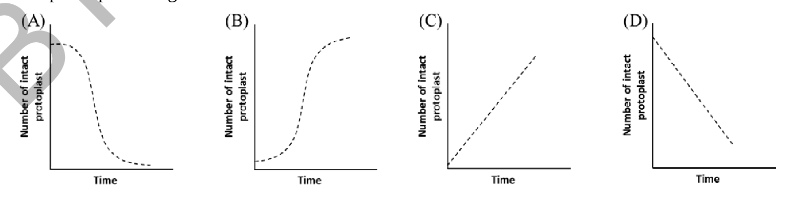
\includegraphics[width=0.5\linewidth]{figs/fig4.png}
    \caption{ }
    \label{fig4}
\end{figure}

\item Which of the following statements with respect to the orientation of the nitrogenous bases to the deoxyribose sugars, and the puckering of the sugar, is correct?  
\hfill \textbf{(GATE EE 2025)}

\begin{enumerate}
\item Anti, and 2$'$-endo in A form DNA  
\item Anti, and 2$'$-endo in B form DNA  
\item Syn, and 3$'$-endo in A form DNA  
\item Syn, and 3$'$-endo in B form DNA  
\end{enumerate}


\item A dioecious plant has XX sexual genotype for female and XY for male. After double fertilization, what would be the genotype of the embryos and endosperm?  
\hfill \textbf{(GATE EE 2025)}

\begin{enumerate}
\item 100\% ovules will have XXX endosperm and XX embryo  
\item 100\% ovules will have XXY endosperm and XY embryo  
\item 50\% ovules will have XXY endosperm and XY embryo, while other 50\% will have XXY endosperm and YY embryo  
\item 50\% ovules will have XXX endosperm and XX embryo, while the other 50\% will have XXY endosperm and XY embryo  
\end{enumerate}


\item The amino acid substitution matrices in decreasing order of stringency for comparing protein sequences are  
\hfill \textbf{(GATE EE 2025)}

\begin{enumerate}
\item PAM250, PAM120, PAM100  
\item PAM100, PAM120, PAM250  
\item PAM250, PAM100, PAM120  
\item PAM120, PAM250, PAM100  
\end{enumerate}


\item The active site in the alpha/beta barrel structures is usually located  
\hfill \textbf{(GATE EE 2025)}

\begin{enumerate}
\item inside the barrel  
\item at the amino side of the strands  
\item at the carboxy side of the strands  
\item at any arbitrary site  
\end{enumerate}


\end{enumerate}

\end{document}


